\chapter{نتایج و ارزیابی}
\section{مقدمه}
سیستم تشخیص حرکات دست به نقش مهمی در ایجاد تعامل کارآمد بین انسان و ماشین تبدیل شده است. پیاده‌سازی این سیستم با استفاده از تشخیص ژست دست، نوید گستره وسیعی از کاربردها را در صنعت فناوری می‌دهد. در این پروژه، 
معماری‌های گوناگونی مانند شبکه‌های عصبی پیچشی، شبکه‌های حافظه کوتاه‌مدت بلند، و شبکه‌های عصبی چندلایه مورد آزمایش قرار گرفتند تا بهترین پیاده‌سازی برای تشخیص حرکات دست انتخاب شود. 
\\
در این فصل، به بررسی نتایج به‌دست‌آمده از این پروژه پیاده‌سازی شده می‌پردازیم و دقت و عملکرد سیستم در شرایط مختلف را ارزیابی می‌کنیم. همچنین، نقاط قوت و ضعف هر یک از معماری‌های مورد استفاده 
را تحلیل کرده و پیشنهاداتی برای بهبود سیستم ارائه خواهیم داد. هدف این فصل، ارائه یک تحلیل جامع از کارایی سیستم و شناخت دقیق‌تر از عواملی است که می‌توانند به ارتقاء عملکرد آن کمک کنند.


\section{ارزیابی عملکرد مدل‌ها}

این پروژه با مدل‌های گوناگونی پیاده‌سازی شد تا بتوان بهترین آنها را برای نتیجه نهایی بر روی پهپاد اجرا کرد. معیارهای ارزیابی شامل دقت، صحت \LTRfootnote{Precision}، فراخوانی\LTRfootnote{Recall}، امتیاز \lr{F1} و
تعداد نمونه‌ها برای هر یک از ژست‌ها می‌باشد.
\\
معیار‌های دقت، صحت، فراخوانی و امتیاز \lr{F1} معیارهای ضروری برای ارزیابی عملکرد مدل یادگیری ماشینی هستند. آنها هر دو مثبت کاذب و منفی کاذب را در نظر
می گیرند و درک دقیقی از قابلیت های پیش بینی یک مدل ارائه می دهند. این ارزیابی دقیق با برجسته کردن نقاط قوت و ضعف خاص به اصلاح مدل کمک می کند.


\subsection{دقت}
دقت مدل معیاری است که نشان می‌دهد یک مدل یادگیری ماشینی چقدر قادر به پیش‌بینی یا تصمیم‌گیری بر اساس داده‌ها است. این معیار به صورت مجموع مثبت و منفی واقعی تقسیم بر تعداد کل نمونه ها محاسبه می شود.
\\
دقت بصری ترین معیار عملکرد است و برابر نسبت مشاهدات پیش بینی شده درست به کل مشاهدات است. این معیار می‌تواند برای مقایسه عملکرد مدل‌های مختلف یا ارزیابی اثربخشی یک مدل خاص برای یک کار معین استفاده شود.
\\
دقت به صورت مجموع مثبت و منفی واقعی تقسیم بر تعداد کل نمونه ها محاسبه می شود. همچنین این معیار زمانی مناسب است که کلاس ها به خوبی متعادل باشند و هزینه های مثبت کاذب و منفی کاذب مشابه باشد.
\[ Accuracy = \frac{True \, Positive + True \, Negative}{True \, Positive + True \, Negative +  False \, Positive + False \, Negative} \]

\begin{table}[h!]
    \centering
    \begin{tabular}{||c c c c||}
     \hline
     \rule{0pt}{3ex} معماری مدل & دوره\LTRfootnote{Epoch} & دقت داده آموزش & دقت داده تست  \\ [1.5ex]
     \hline
     \hline
     \rule{0pt}{0.5ex} & & & \\  
     \lr{MLP} & 6 & 7 & 1 \\ [2.5ex]
     \lr{CNN} & 7 & 8 & 2 \\ [2.5ex]
     \lr{LSTM} & 5 & 8 & 3 \\ [2.5ex]
     \hline
    \end{tabular}
    \caption{جدول ارزیابی دقت مدل‌ها}
    \label{table:2}
\end{table}


\subsection{صحت}
صحت یک معیار آماری برای ارزیابی کیفیت یک مدل پیش‌بینی است. این یکی از معیارهای کلیدی است که برای تعیین عملکرد یک مدل، به ویژه در وظایف طبقه بندی استفاده می شود. صحت نسبت مثبت واقعی به مجموع مثبت های واقعی و مثبت کاذب (نمونه هایی که به اشتباه به عنوان مثبت شناسایی شده اند) است.
\\
صحت بالا نشان دهنده این است که یک مدل در جلوگیری از مثبت کاذب خوب عمل می‌کند، به عنوان مثال، نمونه های منفی را به عنوان مثبت طبقه بندی نمی کند. این امر به ویژه در برنامه هایی که هزینه مثبت کاذب بالا است، اهمیت دارد. 

\[ Precision = \frac{True \, Positive}{True \, Positive - False \, Positive} \]

\subsection{فراخوانی}
معیار فراخوانی که به عنوان نرخ مثبت واقعی نیز شناخته می‌شود، این معیار برابر نمونه‌های داده‌ای است که یک مدل یادگیری ماشینی به درستی آن‌ها را تشخیص داده نسبت به کل نمونه‌های آن کلاس است.
\\
فراخوانی زمانی استفاده می‌شود که به حداقل رساندن منفی های کاذب از اهمیت ویژه ای برخوردار باشد. بدین صورت که هزینه بر روی مثبت کاذب کم باشد و یا هزینه از دست دادن مثبت واقعی زیاد باشد. 
\[ Recall = \frac{True \, Positive}{True \, Positive - False \, Negative} \]

\subsection{امتیاز \lr{F1}}
امتیاز \lr{F1} معیاری برای میانگین هارمونیک دقت و یادآوری است. امتیاز \lr{F1} که معمولاً به عنوان معیار ارزیابی در طبقه‌بندی باینری و چند کلاسه استفاده می‌شود، صحت و یادآوری را در یک متریک واحد ادغام می‌کند تا درک بهتری از عملکرد مدل به دست آورد.
\\
امتیاز \lr{F1} یک معیار مفید برای اندازه‌گیری عملکرد مدل‌های طبقه‌بندی برای زمانی است که داده‌ها نامتعادل‌اند، زیرا نوع خطاها - مثبت کاذب و منفی کاذب - و نه فقط تعداد پیش‌بینی‌های نادرست را در نظر می‌گیرد.


\[ F1  = \frac{2 \times Precision \times Recall}{Precision + Recall} \]



\subsection{گزارش معیارهای ارزیابی در مدل‌ها}
در این بخش، نتایج ارزیابی مدل‌ها برای تشخیص ۹ ژست مختلف دست ارائه شده است.

\begin{figure}[h]
    \centering
    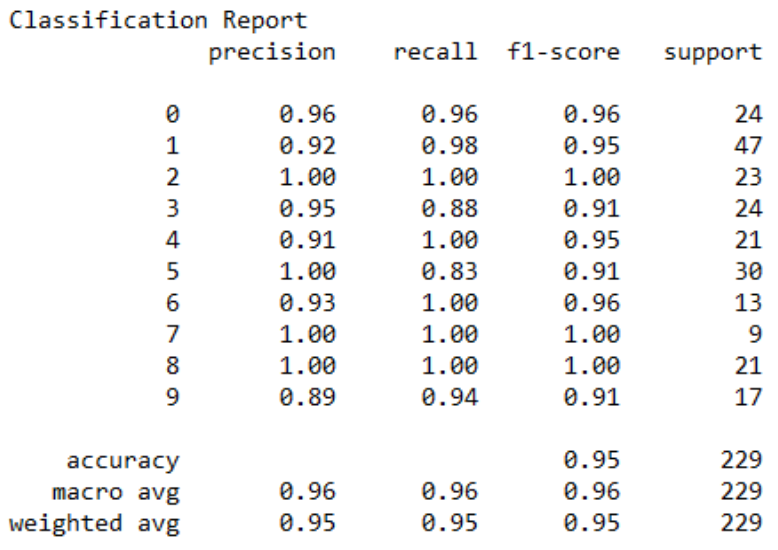
\includegraphics[width=0.7\textwidth]{textchart.png}
    \caption{ معیارهای ارزیابی برای تشخیص ژست دست در مدل \lr{MLP}}
\end{figure}



\section{نمودار‌های دقت و خطا بر حسب دوره}
% بررسی و تحلیل نرخ خطاها
% دلایل خطا و راهکارهای پیشنهادی برای کاهش آنها
یک دوره زمانی است که کل مجموعه داده تنها یک بار از طریق شبکه عصبی به جلو و عقب منتقل می‌شود. از آنجایی که یک دوره آنقدر بزرگ است که نمی‌توان آن را به یکباره به سیستم وارد کرد، آن را به چند دسته کوچکتر تحت عنوان دوره 
تقسیم می‌کنیم.  انتقال کل مجموعه داده از طریق یک شبکه عصبی کافی نبوده و باید مجموعه داده را چندین بار به یک شبکه عصبی ارسال کرد. ما برای این پروژه از یک مجموعه داده محدود استفاده می کنیم و برای بهینه سازی یادگیری آن از گرادیان کاهشی استفاده می‌کنیم. 
\\
تعیین تعداد درست دوره از اهمیت بالایی برخوردار است. با افزایش تعداد دوره‌ها،‌ تعداد دفعات تغییر وزن در شبکه عصبی بیشتر می‌شود و منحنی از کم‌برازش\LTRfootnote{Underfitting} به منحنی بهینه\LTRfootnote{Optimal} و بعد به 
منحنی بیش‌برازش \LTRfootnote{Overfitting} می‌رود. میزان دوره‌ها باید به گونه‌ای تعیین شوند که متعادل عمل کنند و بتوان منحنی را به بهینه ترین حالت ممکن رساند.

\begin{figure}[h]
    \centering
    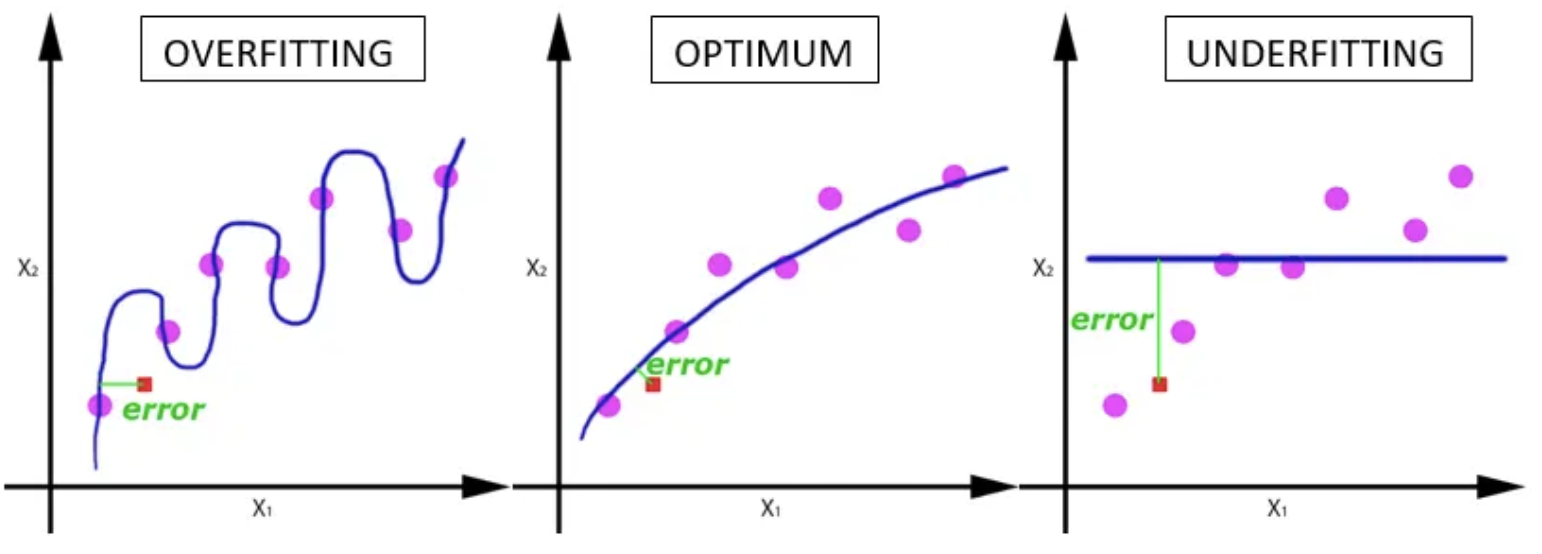
\includegraphics[width=1\textwidth]{fitting.png}
    \caption{منحنی‌های کم‌برازش، بهینه و بیش‌برازش}
\end{figure}


\begin{figure}[h]
    \centering
    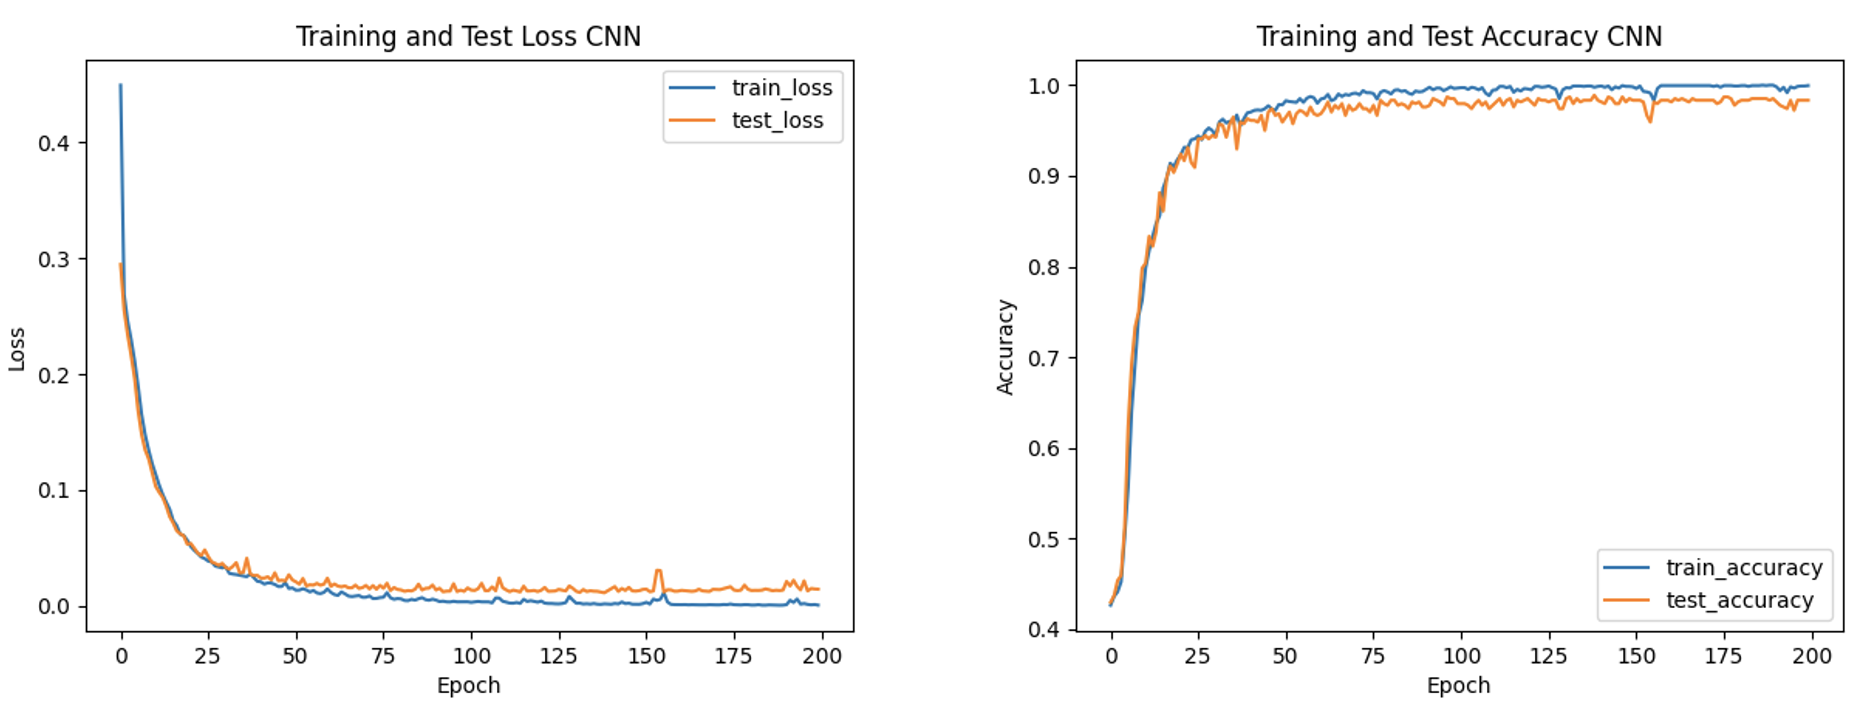
\includegraphics[width=1\textwidth]{CNN.png}
    \caption{نمودار روند دقت و خطا بر حسب دوره در داده‌های آموزش و تست در مدل \lr{CNN}}
\end{figure}


\section{سرعت اجرای برنامه}
از آنجایی که یکی از بزرگ‌ترین اهداف این پروژه زمان واقعی بودن آن است باید میزان پاسخگویی مدل را نیز در نظر قرار داد. در جدول زیر زمان پاسخ‌گویی مدل ها از زمانی که داده‌ها از طریق دوربین خوانده می‌شوند تا زمانی که دستور به پهپاد داده‌ می‌شود نشان داده‌شده.

\begin{table}[h!]
    \centering
    \begin{tabular}{||c c||}
     \hline
     \rule{0pt}{3ex}معماری مدل & زمان پاسخگویی مدل\\ [1.5ex]
     \hline
     \hline
     \rule{0pt}{0.5ex} & \\  % Adds space before the first data row, while keeping the vertical lines
     \lr{MLP} & 6 \\ [2.5ex]
     \lr{CNN} & 7 \\ [2.5ex]
     \lr{LSTM} & 5 \\ [2.5ex]
     \hline
    \end{tabular}
    \caption{جدول ارزیابی زمان پاسخگویی مدل‌ها}
    \label{table:1}
\end{table}


\section{سخت‌افزار مورد نیاز}
این پروژه باید به گونه‌ای اجرا می‌شد که بر روی ساده‌ترین سیستم‌های کامپیوتری نیز قابل اجرا باشد، زیرا سخت‌افزار پهپادها به‌طور معمول دارای پردازنده‌های ضعیف‌تری هستند. همچنین، استفاده از کارت گرافیکی ممکن نبود، چرا که 
پهپادها فاقد کارت گرافیکی می‌باشند. معماری‌های پیاده‌سازی شده به نحوی طراحی شدند که تعادل میان دقت و بهره‌وری از سخت‌افزار حفظ شود، به طوری که هم قابلیت اجرای زمان واقعی داشته باشند و هم امکان پیاده‌سازی آن‌ها بر روی پهپاد 
فراهم باشد. از این رو، معماری‌ها به گونه‌ای پیاده‌سازی شدند که بر روی پردازنده اجرا شوند و میزان استفاده از پردازنده برای آن‌ها به شرح زیر است:


\begin{table}[h!]
    \centering
    \begin{tabular}{||c c c||}
     \hline
     \rule{0pt}{3ex}معماری مدل & پردازنده & فضای ذخیره‌شده \\ [1.5ex]
     \hline
     \hline
     \rule{0pt}{0.5ex} & & \\  % Adds space before the first data row, while keeping the vertical lines
     \lr{MLP} & 6 & 7 \\ [2.5ex]
     \lr{CNN} & 7 & 8 \\ [2.5ex]
     \lr{LSTM} & 5 & 8 \\ [2.5ex]
     \hline
    \end{tabular}
    \caption{جدول ارزیابی سخت‌افزار موردنیاز مدل‌ها}
    \label{table:1}
\end{table}


\section{مقایسه دقت پروژه ما با کارهای مشابه}
پروژه پیاده‌سازی از دقت بسیار بالایی برخوردار است که این دقت به دلیل ترکیب پیش‌پردازش، کتابخانه \lr{MediaPipe}، مدل کلاس‌بندی و پس‌پردازش است. 
\\ در این قسمت به مقایسه دقت پروژه پیاده‌سازی شده با پروژه‌های مشابه با هدف کنترل پهپاد با کمک تشخیص ژست دست پرداخته‌ایم.

\begin{table}[h!]
    \centering
    \begin{tabular}{||>{\centering\arraybackslash}p{10.5cm} >{\centering\arraybackslash}p{2cm} >{\centering\arraybackslash}p{2cm}||}
     \hline
     \rule{0pt}{3ex} نام مقاله & تعداد ژست‌های دست & دقت تشخیص ژست دست \\ [1.5ex]
     \hline
     \rule{0pt}{0.5ex} & & \\  
     برنامه ما & 9 & 6 \\ [2.5ex]
     \lr{Hand Gesture Controlled Drones: An Open Source Library\cite{natarajan2018hand}} & 5 & ۴۷۱.۹۷ \\ [2.5ex]
     \lr{A real-time hand gesture recognition method\cite{fang2007real}} & 6 & 8.93 \\ [2.5ex]
     \lr{Hand Gestures For Drone Control Using Deep Learning\cite{hadri2018hand}} & 9 & 3.83  \\ [2.5ex]
     \lr{UAV-GESTURE: A Dataset for UAV Control and Gesture Recognition\cite{perera2018uav}} & 13 & 9.91 \\ [2.5ex]
     \lr{Hand Gesture Recognition system for Real-Time Application\cite{murugeswari2014hand}} & 6 & 8.90 \\ [2.5ex]
     \lr{An improved hand gesture recognition system using keypoints and hand bounding boxes\cite{dang2022improved}} & 6 & 94 \\ [2.5ex]
     \lr{Hand-gesture recognition using computer-vision techniques\cite{rios2013hand}} & 6 & 1.93 \\ [2.5ex]
     \lr{Hand Gesture Recognition using Image Processing and Feature Extraction Techniques\cite{sharma2020hand}} & 28 & 54.89 \\ [2.5ex]
     \lr{Applying Hand Gesture Recognition for User Guide Application Using MediaPipe\cite{harris2021applying}} & 10 & 95 \\ [2.5ex]
     \lr{MediaPipe Hands: On-device Real-time Hand Tracking\cite{zhang2020mediapipe}} & 8 & 7.94 \\ [2.5ex]
     \lr{Hand Gesture Recognition System based in Computer Vision and Machine Learning\cite{trigueiros2015hand}} & 28 & 72.93 \\ [2.5ex]
     \lr{Hand Gesture Recogrution Using Hidden Markov Models\cite{min1997hand}} & 5 & 1.92 \\ [2.5ex]
     \lr{Hand gesture recognition using Kinect\cite{li2012hand}} & 38 & 84 \\ [2.5ex]
     \lr{Hand gesture recognition using neural networks\cite{murthy2010hand}} & 10 & 89 \\ [2.5ex]
     \hline
    \end{tabular}
    \caption{جدول مقایسه پروژه با کارهای مشابه}
\end{table}



\section{جمع‌بندی}
مدل‌هایی که در این پروژه ارائه شده‌اند، دارای دقت و کارایی مناسبی هستند که امکان استفاده آن‌ها در کاربردهای واقعی را فراهم می‌کند. به عبارت دیگر، این مدل‌ها می‌توانند به خوبی ژست‌های دست را تشخیص داده و از آن‌ها در عملیات مختلفی مانند کنترل دستگاه‌ها و رابط‌های کاربری استفاده شود.
\\
علاوه بر این، با مقایسه عملکرد پروژه ما با کارهای مشابه در حوزه تشخیص ژست‌های دست، مشخص شده است که پروژه ما در مقایسه با آن‌ها دارای دقت مشابه یا حتی بالاتری است، به ویژه اگر تعداد کلاس‌های ژست دست در نظر گرفته 
شود. این نکته نشان می‌دهد که مدل‌هایی که در این پروژه ارائه شده‌اند، به خوبی تنوع و پیچیدگی ژست‌های دست درک می‌کنند و قادر به تشخیص آن‌ها هستند، که این امر یکی از چالش‌های اصلی در این زمینه است.
\\
با توجه به این نتایج، می‌توانیم اطمینان داشته باشیم که پروژه ما قادر است به عنوان یک راه‌حل کارآمد برای تشخیص ژست‌های دست در برنامه‌ها و سیستم‌های واقعی مورد استفاده قرار بگیرد.
